%------------------
\section{Enumeration Case Studies\label{sec:ch2:simple}}

In this section, a number of case studies are provided to demonstrate the theoretical aspects of the previous sections\footnote{Ref.~\cite{github-pm-architectures-project} contains \xprog{Matlab} codes that replicate the results from these enumeration case studies and can generate graphs for $(C,R,P)$ architecture design problems.}.

\subsection{Case Study 1\label{sec:ch2:example1}}

\begin{figure}
\centering

\tikzsetnextfilename{cpexamples}

\begin{subfigure}[b]{1\columnwidth}
\centering
% \cfbox{box-gray}{
\resizebox{!}{12mm}{
\begin{tikzpicture}[
mynode/.style={draw, circle, very thick, inner sep=1pt, scale=1.3},
myline/.style={draw, very thick},
]

\node[mynode,draw=red] (1) at (-2,-0) {$\xcolor{R}_1^1$};
\node[mynode,draw=red] (2) at (-1,-1) {$\xcolor{R}_2^1$};
\node[mynode,draw=red] (3) at (0,0) {$\xcolor{R}_3^1$};
\node[mynode,draw=ForestGreen] (4) at (1,-1) {$\xcolor{G}_1^1$};
\node[mynode,draw=ForestGreen] (5) at (2,0) {$\xcolor{G}_1^2$};
\node[mynode,draw=ForestGreen] (6) at (3,-1) {$\xcolor{G}_2^1$};
\node[mynode,draw=ForestGreen] (7) at (4,0) {$\xcolor{G}_2^2$};
\node[mynode,draw=blue] (8) at (5,-1) {$\xcolor{B}_1^1$};
\node[mynode,draw=blue] (9) at (6,0) {$\xcolor{B}_1^2$};
\node[mynode,draw=blue] (10) at (7,-1) {$\xcolor{B}_1^3$};

\draw [myline] (4) -- (5);
\draw [myline] (6) -- (7);
\draw [myline] (8) -- (9);
\draw [myline] (8) -- (10);
\draw [myline] (9) -- (10);

\end{tikzpicture}
}
% } 
\caption{\nameref{sec:ch2:example1}. \label{fig:ch2:cpexamples:1}}
\end{subfigure}

\begin{subfigure}[b]{1\columnwidth}
\centering
% \cfbox{box-gray}{
\resizebox{!}{12mm}{
\begin{tikzpicture}[
mynode/.style={draw, circle, very thick, inner sep=1pt, scale=1.3},
myline/.style={draw, very thick},
]

\node[mynode,draw=Purple] (1) at (-2,0) {$\xcolor{P}_1^1$};
\node[mynode,draw=red] (2) at (-1,-1) {$\xcolor{R}_1^1$};
\node[mynode,draw=red] (3) at (0,0) {$\xcolor{R}_2^1$};
\node[mynode,draw=ForestGreen] (4) at (1,-1) {$\xcolor{G}_1^1$};
\node[mynode,draw=ForestGreen] (5) at (2,0) {$\xcolor{G}_1^2$};
\node[mynode,draw=ForestGreen] (6) at (3,-1) {$\xcolor{G}_2^1$};
\node[mynode,draw=ForestGreen] (7) at (4,0) {$\xcolor{G}_2^2$};
\node[mynode,draw=blue] (8) at (5,-1) {$\xcolor{B}_1^1$};
\node[mynode,draw=blue] (9) at (6,0) {$\xcolor{B}_1^2$};
\node[mynode,draw=blue] (10) at (7,-1) {$\xcolor{B}_1^3$};
\node[mynode,draw=YellowOrange] (11) at (8,0) {$\xcolor{O}_1^1$};
\node[mynode,draw=YellowOrange] (12) at (9,-1) {$\xcolor{O}_1^2$};
\node[mynode,draw=YellowOrange] (13) at (10,0) {$\xcolor{O}_1^3$};
\node[mynode,draw=YellowOrange] (14) at (11,-1) {$\xcolor{O}_1^4$};

\draw [myline] (4) -- (5);
\draw [myline] (6) -- (7);
\draw [myline] (8) -- (9);
\draw [myline] (8) -- (10);
\draw [myline] (9) -- (10);
\draw [myline] (11) -- (12);
\draw [myline] (11) -- (13);
\draw [myline] (12) -- (13);
\draw [myline] (11) -- (14);
\draw [myline] (12) -- (14);
\draw [myline] (13) -- (14);

\end{tikzpicture}
}
% }
\caption{\nameref{sec:ch2:example2}. \label{fig:ch2:cpexamples:2}}
\end{subfigure}

\caption{$G^{P}$ graphs for two examples. \label{fig:cpexamples}}

\end{figure}



\begin{figure}
\centering

\begin{subfigure}[b]{0.25\columnwidth}
\centering
\cfbox{box-gray}{
\resizebox{!}{\textwidth}{
\tikzsetnextfilename{inter11}
\begin{tikzpicture}[
mynode/.style={draw, circle, very thick, inner sep=1pt, scale=1.3},
myline/.style={draw, very thick},
]
\pgfmathsetmacro{\n}{10};
\pgfmathsetmacro{\r}{2.5};

\node[mynode,draw=red] (1) at (0*360/\n + 90: \r cm) {$\xcolor{R}_1^1$};
\node[mynode,draw=red] (2) at (1*360/\n + 90: \r cm) {$\xcolor{R}_2^1$};
\node[mynode,draw=red] (3) at  (2*360/\n + 90: \r cm) {$\xcolor{R}_3^1$};
\node[mynode,draw=ForestGreen] (4) at  (3*360/\n + 90: \r cm) {$\xcolor{G}_1^1$};
\node[mynode,draw=ForestGreen] (5) at  (4*360/\n + 90: \r cm) {$\xcolor{G}_1^2$};
\node[mynode,draw=ForestGreen] (6) at  (5*360/\n + 90: \r cm) {$\xcolor{G}_2^1$};
\node[mynode,draw=ForestGreen] (7) at  (6*360/\n + 90: \r cm) {$\xcolor{G}_2^2$};
\node[mynode,draw=blue] (8) at  (7*360/\n + 90: \r cm) {$\xcolor{B}_1^1$};
\node[mynode,draw=blue] (9) at  (8*360/\n + 90: \r cm) {$\xcolor{B}_1^2$};
\node[mynode,draw=blue] (10) at  (9*360/\n + 90: \r cm) {$\xcolor{B}_1^3$};

\foreach \i in {1,...,\n}{
	\foreach \j in {\i,...,\n}{
    	\draw [myline,light-gray] (\i) -- (\j);
} }

\end{tikzpicture}
}
}
\caption{$K_{10}$.\label{fig:ch2:inter1_1}}
\end{subfigure}
%
% \hspace{0.02\textwidth}
%
\begin{subfigure}[b]{0.25\columnwidth}
\centering
\cfbox{box-gray}{
\resizebox{!}{\textwidth}{
\tikzsetnextfilename{inter12}
\begin{tikzpicture}[
mynode/.style={draw, circle, very thick, inner sep=1pt, scale=1.3},
myline/.style={draw, very thick},
]
\pgfmathsetmacro{\n}{10};
\pgfmathsetmacro{\r}{2.5};

\node[mynode,draw=red] (1) at (0*360/\n + 90: \r cm) {$\xcolor{R}_1^1$};
\node[mynode,draw=red] (2) at (1*360/\n + 90: \r cm) {$\xcolor{R}_2^1$};
\node[mynode,draw=red] (3) at  (2*360/\n + 90: \r cm) {$\xcolor{R}_3^1$};
\node[mynode,draw=ForestGreen] (4) at  (3*360/\n + 90: \r cm) {$\xcolor{G}_1^1$};
\node[mynode,draw=ForestGreen] (5) at  (4*360/\n + 90: \r cm) {$\xcolor{G}_1^2$};
\node[mynode,draw=ForestGreen] (6) at  (5*360/\n + 90: \r cm) {$\xcolor{G}_2^1$};
\node[mynode,draw=ForestGreen] (7) at  (6*360/\n + 90: \r cm) {$\xcolor{G}_2^2$};
\node[mynode,draw=blue] (8) at  (7*360/\n + 90: \r cm) {$\xcolor{B}_1^1$};
\node[mynode,draw=blue] (9) at  (8*360/\n + 90: \r cm) {$\xcolor{B}_1^2$};
\node[mynode,draw=blue] (10) at  (9*360/\n + 90: \r cm) {$\xcolor{B}_1^3$};

\draw [myline] (10) -- (1);
\draw [myline] (9) -- (2);
\draw [myline] (8) -- (3);
\draw [myline] (7) -- (4);
\draw [myline] (6) -- (5);

\end{tikzpicture}
}
}
\caption{\mypm{}~1.\label{fig:ch2:inter1_2}}
\end{subfigure}
%
% \hspace{0.02\textwidth}
%
\begin{subfigure}[b]{0.25\columnwidth}
\centering
\cfbox{box-gray}{
\resizebox{!}{\textwidth}{
\tikzsetnextfilename{inter13}
\begin{tikzpicture}[
mynode/.style={draw, circle, very thick, inner sep=1pt, scale=1.3},
myline/.style={draw, very thick},
]
\pgfmathsetmacro{\n}{10};
\pgfmathsetmacro{\r}{2.5};

\node[mynode,draw=red] (1) at (0*360/\n + 90: \r cm) {$\xcolor{R}_1^1$};
\node[mynode,draw=red] (2) at (1*360/\n + 90: \r cm) {$\xcolor{R}_2^1$};
\node[mynode,draw=red] (3) at  (2*360/\n + 90: \r cm) {$\xcolor{R}_3^1$};
\node[mynode,draw=ForestGreen] (4) at  (3*360/\n + 90: \r cm) {$\xcolor{G}_1^1$};
\node[mynode,draw=ForestGreen] (5) at  (4*360/\n + 90: \r cm) {$\xcolor{G}_1^2$};
\node[mynode,draw=ForestGreen] (6) at  (5*360/\n + 90: \r cm) {$\xcolor{G}_2^1$};
\node[mynode,draw=ForestGreen] (7) at  (6*360/\n + 90: \r cm) {$\xcolor{G}_2^2$};
\node[mynode,draw=blue] (8) at  (7*360/\n + 90: \r cm) {$\xcolor{B}_1^1$};
\node[mynode,draw=blue] (9) at  (8*360/\n + 90: \r cm) {$\xcolor{B}_1^2$};
\node[mynode,draw=blue] (10) at  (9*360/\n + 90: \r cm) {$\xcolor{B}_1^3$};

\draw [myline] (10) -- (5);
\draw [myline] (9) -- (3);
\draw [myline] (8) -- (6);
\draw [myline] (7) -- (4);
\draw [myline] (2) -- (1);

\end{tikzpicture}
}
}
\caption{\mypm{}~462.\label{fig:ch2:inter1_3}}
\end{subfigure}


\caption{Select interconnectivity graphs for \nameref{sec:ch2:example1}.\label{fig:ch2:inter1}}

\end{figure}

% \draw [] (10) -- (9);
% \draw [] (8) -- (2);
% \draw [] (7) -- (4);
% \draw [] (6) -- (5);
% \draw [] (3) -- (1);
% \caption{ 864 of 945 }

\begin{figure}
\centering

\begin{subfigure}[b]{0.25\columnwidth}
\centering
\cfbox{box-gray}{
\resizebox{!}{\textwidth}{
\tikzsetnextfilename{model1_1}
\begin{tikzpicture}[
mynode/.style={draw, circle, very thick, inner sep=1pt, scale=1.3},
myline/.style={draw, very thick},
]
\pgfmathsetmacro{\n}{10};
\pgfmathsetmacro{\r}{2.5};

\node[mynode,draw=red] (1) at (0*360/\n + 90: \r cm) {$\xcolor{R}_1^1$};
\node[mynode,draw=red] (2) at (1*360/\n + 90: \r cm) {$\xcolor{R}_2^1$};
\node[mynode,draw=red] (3) at  (2*360/\n + 90: \r cm) {$\xcolor{R}_3^1$};
\node[mynode,draw=ForestGreen] (4) at  (3*360/\n + 90: \r cm) {$\xcolor{G}_1^1$};
\node[mynode,draw=ForestGreen] (5) at  (4*360/\n + 90: \r cm) {$\xcolor{G}_1^2$};
\node[mynode,draw=ForestGreen] (6) at  (5*360/\n + 90: \r cm) {$\xcolor{G}_2^1$};
\node[mynode,draw=ForestGreen] (7) at  (6*360/\n + 90: \r cm) {$\xcolor{G}_2^2$};
\node[mynode,draw=blue] (8) at  (7*360/\n + 90: \r cm) {$\xcolor{B}_1^1$};
\node[mynode,draw=blue] (9) at  (8*360/\n + 90: \r cm) {$\xcolor{B}_1^2$};
\node[mynode,draw=blue] (10) at  (9*360/\n + 90: \r cm) {$\xcolor{B}_1^3$};


\draw [myline] (10) -- (1);
\draw [myline] (9) -- (2);
\draw [myline] (8) -- (3);
\draw [myline] (7) -- (4);
\draw [myline] (6) -- (5);

\draw [myline] (4) -- (5);
\draw [myline] (6) -- (7);
\draw [myline] (8) -- (9);
\draw [myline] (8) -- (10);
\draw [myline] (9) -- (10);

\end{tikzpicture}
}
}
\caption{$G^{CP}$  for  \mypm{}~1.\label{fig:ch2:model1_1}}
\end{subfigure}
%
% \hspace{0.02\textwidth}
%
\begin{subfigure}[b]{0.25\columnwidth}
\centering
\cfbox{box-gray}{
\resizebox{!}{\textwidth}{
\tikzsetnextfilename{model1_2}
\begin{tikzpicture}[
mynode/.style={draw, circle, very thick, inner sep=1pt, scale=1.3},
myline/.style={draw, very thick},
]
\pgfmathsetmacro{\n}{6};
\pgfmathsetmacro{\r}{1.5};

\node[mynode,draw=red] (1) at (0*360/\n + 90: \r cm) {$\xcolor{R}$};
\node[mynode,draw=red] (2) at (1*360/\n + 90: \r cm) {$\xcolor{R}$};
\node[mynode,draw=red] (3) at  (2*360/\n + 90: \r cm) {$\xcolor{R}$};
\node[mynode,draw=ForestGreen] (4) at  (3*360/\n + 90: \r cm) {$\xcolor{G}$};
\node[mynode,draw=ForestGreen] (5) at  (4*360/\n + 90: \r cm) {$\xcolor{G}$};
\node[mynode,draw=blue, circle] (6) at  (5*360/\n + 90: \r cm) {$\xcolor{B}$};

\draw [myline] (1) -- (6);
\draw [myline] (2) -- (6);
\draw [myline] (3) -- (6);
\draw [myline] (4) -- (5);

\end{tikzpicture}
}
}
\caption{$G^{CC}$  for  \mypm{}~1.\label{fig:ch2:model1_2}}
\end{subfigure}
%
% \hspace{0.02\textwidth}
%
%\begin{subfigure}[b]{0.32\columnwidth}
%\centering
%\cfbox{box-gray}{
%\resizebox{!}{\textwidth}{
%\tikzsetnextfilename{model1_3}
%\begin{tikzpicture}[
%mynode/.style={draw, circle, very thick, inner sep=1pt, scale=1.3},
%myline/.style={draw, very thick},
%]
%\pgfmathsetmacro{\n}{10};
%\pgfmathsetmacro{\r}{2.5};
%
%\node[mynode,draw=red] (1) at (0*360/\n + 90: \r cm) {$\xcolor{R}_1^1$};
%\node[mynode,draw=red] (2) at (1*360/\n + 90: \r cm) {$\xcolor{R}_2^1$};
%\node[mynode,draw=red] (3) at  (2*360/\n + 90: \r cm) {$\xcolor{R}_3^1$};
%\node[mynode,draw=ForestGreen] (4) at  (3*360/\n + 90: \r cm) {$\xcolor{G}_1^1$};
%\node[mynode,draw=ForestGreen] (5) at  (4*360/\n + 90: \r cm) {$\xcolor{G}_1^2$};
%\node[mynode,draw=ForestGreen] (6) at  (5*360/\n + 90: \r cm) {$\xcolor{G}_2^1$};
%\node[mynode,draw=ForestGreen] (7) at  (6*360/\n + 90: \r cm) {$\xcolor{G}_2^2$};
%\node[mynode,draw=blue] (8) at  (7*360/\n + 90: \r cm) {$\xcolor{B}_1^1$};
%\node[mynode,draw=blue] (9) at  (8*360/\n + 90: \r cm) {$\xcolor{B}_1^2$};
%\node[mynode,draw=blue] (10) at  (9*360/\n + 90: \r cm) {$\xcolor{B}_1^3$};
%
%
%\draw [myline] (10) -- (5);
%\draw [myline] (9) -- (3);
%\draw [myline] (8) -- (6);
%\draw [myline] (7) -- (4);
%\draw [myline] (2) -- (1);
%
%\draw [myline] (4) -- (5);
%\draw [myline] (6) -- (7);
%\draw [myline] (8) -- (9);
%\draw [myline] (8) -- (10);
%\draw [myline] (9) -- (10);
%
%\end{tikzpicture}
%}
%}
%\caption{$G^{CP}$  for  \mypm{}~462.\label{fig:model1_3}}
%\end{subfigure}
%%
%\hspace{0.02\textwidth}
%%
\begin{subfigure}[b]{0.25\columnwidth}
\centering
\cfbox{box-gray}{
\resizebox{!}{\textwidth}{
\tikzsetnextfilename{model1_4}
\begin{tikzpicture}[
mynode/.style={draw, circle, very thick, inner sep=1pt, scale=1.3},
myline/.style={draw, very thick},
]
\pgfmathsetmacro{\n}{6};
\pgfmathsetmacro{\r}{1.5};

\node[mynode,draw=red] (1) at (0*360/\n + 90: \r cm) {$\xcolor{R}$};
\node[mynode,draw=red] (2) at (1*360/\n + 90: \r cm) {$\xcolor{R}$};
\node[mynode,draw=red] (3) at  (2*360/\n + 90: \r cm) {$\xcolor{R}$};
\node[mynode,draw=ForestGreen] (4) at  (3*360/\n + 90: \r cm) {$\xcolor{G}$};
\node[mynode,draw=ForestGreen] (5) at  (4*360/\n + 90: \r cm) {$\xcolor{G}$};
\node[mynode,draw=blue, circle] (6) at  (5*360/\n + 90: \r cm) {$\xcolor{B}$};

\draw [myline] (1) -- (2);
\draw [myline] (3) -- (6);
\draw [myline] (4) -- (6);
\draw [myline] (5) -- (6);
\draw [myline] (5) -- (4);

\end{tikzpicture}
}
}
\caption{$G^{CC}$ for \mypm{}~462.\label{fig:ch2:model1_4}}
\end{subfigure}

\caption{Select connected ports and connected component graphs for \nameref{sec:ch2:example1}.\label{fig:model1}}

\end{figure}

The base three-tuple is specified as:
\begin{align*}
{C} &= \left\lbrace \xcolor{R}, \xcolor{G}, \xcolor{B} \right\rbrace, \qquad {R} = [ 3, 2, 1 ], \qquad {P} = [ 1, 2, 3 ]
\end{align*}

\noindent This example has three different simple component types that have multiple ports and replicates and is visualized in Fig.~\ref{fig:ch2:cpexamples:1}. Then $G^{P}$ is:
\begin{align*}
{V}^{P} &= \left\lbrace  1, 2, 3, 4, 5, 6, 7, 8, 9, 10 \right\rbrace \\
{E}^{P} &= \left\lbrace  (4,5), (6,7), (8,9), (8,10), (9,10) \right\rbrace \\
{L}^{P} &= \left\lbrace \xcolor{R}_1^1, \xcolor{R}_2^1, \xcolor{R}_3^1, \xcolor{G}_1^1, \xcolor{G}_1^2, \xcolor{G}_2^1, \xcolor{G}_2^2, \xcolor{B}_1^1, \xcolor{B}_1^2, \xcolor{B}_1^3 \right\rbrace \\
N_P &= 10, \quad N_C = 6, \quad 3.28 \leq \abs*{\mathcal{G}_3} \leq 945
\end{align*}

\noindent In Fig.~\ref{fig:ch2:inter1} we see $G^{I}$ for two different \mypm{}s. Then in Fig.~\ref{fig:ch2:model1_1} we can see $G^{CP}$ for \mypm{}~1. This can then be mapped to the equivalent $G^{CC}$ shown in Fig.~\ref{fig:ch2:model1_2}. The basic tree search algorithm will have the same tree regardless of the NSCs and this tree is visualized in Fig.~\ref{fig:ch2:tree1simple}. Both graphs in Figs.~\ref{fig:ch2:model1_2} and \ref{fig:ch2:model1_4} will have a topologically equivalent graph appear in the set of graphs generated by this algorithm. Now two different sets of NSCs will be discussed.

\begin{enumerate}[nosep]

\item \label{ch2:example11} No additional NSCs. There are 32,768 adjacency matrices ($\mathcal{G}_0$);  945 \mypm{}s ($\mathcal{G}_1$); 86 candidate graphs with basic tree search algorithm; 77 remaining candidate graphs after initial port-type isomorphism filter; and 77 feasible graphs ($\mathcal{G}_2$). Finally, there are only 16 unique graphs ($\mathcal{G}_3$) consistent with Eqn.~(\ref{eq:ch2:lowerbnd}) and all shown in Fig.~\ref{fig:ch2:unique1}. 258 graph comparisons were needed and only 113 required a full isomorphism check.

\begin{figure*}

\definecolor{R}{rgb}{1,0,0} % red
\definecolor{G}{rgb}{0,0.6,0.36078431372} % forestgreen
\definecolor{B}{rgb}{0,0,1} % blue
\definecolor{O}{rgb}{0.99607843137,0.63529411764,0.22745098039} % orange
\definecolor{P}{rgb}{0.60784313725,0.27843137254,0.58823529411} % purple
\centering
% \newcommand{\uniquesize}{0.115\textwidth}
\newcommand{\uniquesize}{0.14\textwidth}
%
%
%
\begin{subfigure}[b]{\uniquesize}
\centering
\resizebox{!}{\textwidth}{
\begin{tikzpicture}[
mynode/.style={draw, circle, very thick, inner sep=1pt, scale=1.3},
myline/.style={draw, very thick},
]
\pgfmathsetmacro{\n}{6};
\pgfmathsetmacro{\r}{1.5};
\node[mynode,draw=R] (1) at (0*360/\n + 90: \r cm) {$\xcolor{R}$};
\node[mynode,draw=R] (2) at (1*360/\n + 90: \r cm) {$\xcolor{R}$};
\node[mynode,draw=R] (3) at (2*360/\n + 90: \r cm) {$\xcolor{R}$};
\node[mynode,draw=G] (4) at (3*360/\n + 90: \r cm) {$\xcolor{G}$};
\node[mynode,draw=G] (5) at (4*360/\n + 90: \r cm) {$\xcolor{G}$};
\node[mynode,draw=B] (6) at (5*360/\n + 90: \r cm) {$\xcolor{B}$};
\draw [myline] (6) -- (1);
\draw [myline] (6) -- (2);
\draw [myline] (6) -- (3);
\draw [myline] (5) -- (4);
\end{tikzpicture}
}
\caption{\mypm{}~227}
\end{subfigure}
%
%
%
\begin{subfigure}[b]{\uniquesize}
\centering
\resizebox{!}{\textwidth}{
\begin{tikzpicture}[
mynode/.style={draw, circle, very thick, inner sep=1pt, scale=1.3},
myline/.style={draw, very thick},
]
\pgfmathsetmacro{\n}{6};
\pgfmathsetmacro{\r}{1.5};
\node[mynode,draw=R] (1) at (0*360/\n + 90: \r cm) {$\xcolor{R}$};
\node[mynode,draw=R] (2) at (1*360/\n + 90: \r cm) {$\xcolor{R}$};
\node[mynode,draw=R] (3) at (2*360/\n + 90: \r cm) {$\xcolor{R}$};
\node[mynode,draw=G] (4) at (3*360/\n + 90: \r cm) {$\xcolor{G}$};
\node[mynode,draw=G] (5) at (4*360/\n + 90: \r cm) {$\xcolor{G}$};
\node[mynode,draw=B] (6) at (5*360/\n + 90: \r cm) {$\xcolor{B}$};
\draw [myline] (6) -- (1);
\draw [myline] (6) -- (2);
\draw [myline] (6) -- (3);
\end{tikzpicture}
}
\caption{\mypm{}~228}
\end{subfigure}
%
%
%
\begin{subfigure}[b]{\uniquesize}
\centering
\resizebox{!}{\textwidth}{
\begin{tikzpicture}[
mynode/.style={draw, circle, very thick, inner sep=1pt, scale=1.3},
myline/.style={draw, very thick},
]
\pgfmathsetmacro{\n}{6};
\pgfmathsetmacro{\r}{1.5};
\node[mynode,draw=R] (1) at (0*360/\n + 90: \r cm) {$\xcolor{R}$};
\node[mynode,draw=R] (2) at (1*360/\n + 90: \r cm) {$\xcolor{R}$};
\node[mynode,draw=R] (3) at (2*360/\n + 90: \r cm) {$\xcolor{R}$};
\node[mynode,draw=G] (4) at (3*360/\n + 90: \r cm) {$\xcolor{G}$};
\node[mynode,draw=G] (5) at (4*360/\n + 90: \r cm) {$\xcolor{G}$};
\node[mynode,draw=B] (6) at (5*360/\n + 90: \r cm) {$\xcolor{B}$};
\draw [myline] (6) -- (1);
\draw [myline] (6) -- (2);
\draw [myline] (5) -- (3);
\draw [myline] (5) -- (4);
\draw [myline] (6) -- (4);
\end{tikzpicture}
}
\caption{\mypm{}~332}
\end{subfigure}
%
%
%
\begin{subfigure}[b]{\uniquesize}
\centering
\resizebox{!}{\textwidth}{
\begin{tikzpicture}[
mynode/.style={draw, circle, very thick, inner sep=1pt, scale=1.3},
myline/.style={draw, very thick},
]
\pgfmathsetmacro{\n}{6};
\pgfmathsetmacro{\r}{1.5};
\node[mynode,draw=R] (1) at (0*360/\n + 90: \r cm) {$\xcolor{R}$};
\node[mynode,draw=R] (2) at (1*360/\n + 90: \r cm) {$\xcolor{R}$};
\node[mynode,draw=R] (3) at (2*360/\n + 90: \r cm) {$\xcolor{R}$};
\node[mynode,draw=G] (4) at (3*360/\n + 90: \r cm) {$\xcolor{G}$};
\node[mynode,draw=G] (5) at (4*360/\n + 90: \r cm) {$\xcolor{G}$};
\node[mynode,draw=B] (6) at (5*360/\n + 90: \r cm) {$\xcolor{B}$};
\draw [myline] (6) -- (1);
\draw [myline] (6) -- (2);
\draw [myline] (4) -- (3);
\draw [myline] (6) -- (4);
\end{tikzpicture}
}
\caption{\mypm{}~438}
\end{subfigure}
%
%
%
\begin{subfigure}[b]{\uniquesize}
\centering
\resizebox{!}{\textwidth}{
\begin{tikzpicture}[
mynode/.style={draw, circle, very thick, inner sep=1pt, scale=1.3},
myline/.style={draw, very thick},
]
\pgfmathsetmacro{\n}{6};
\pgfmathsetmacro{\r}{1.5};
\node[mynode,draw=R] (1) at (0*360/\n + 90: \r cm) {$\xcolor{R}$};
\node[mynode,draw=R] (2) at (1*360/\n + 90: \r cm) {$\xcolor{R}$};
\node[mynode,draw=R] (3) at (2*360/\n + 90: \r cm) {$\xcolor{R}$};
\node[mynode,draw=G] (4) at (3*360/\n + 90: \r cm) {$\xcolor{G}$};
\node[mynode,draw=G] (5) at (4*360/\n + 90: \r cm) {$\xcolor{G}$};
\node[mynode,draw=B] (6) at (5*360/\n + 90: \r cm) {$\xcolor{B}$};
\draw [myline] (6) -- (1);
\draw [myline] (5) -- (2);
\draw [myline] (5) -- (3);
\draw [myline] (6) -- (4);
\end{tikzpicture}
}
\caption{\mypm{}~467}
\end{subfigure}
%
%
%
\begin{subfigure}[b]{\uniquesize}
\centering
\resizebox{!}{\textwidth}{
\begin{tikzpicture}[
mynode/.style={draw, circle, very thick, inner sep=1pt, scale=1.3},
myline/.style={draw, very thick},
]
\pgfmathsetmacro{\n}{6};
\pgfmathsetmacro{\r}{1.5};
\node[mynode,draw=R] (1) at (0*360/\n + 90: \r cm) {$\xcolor{R}$};
\node[mynode,draw=R] (2) at (1*360/\n + 90: \r cm) {$\xcolor{R}$};
\node[mynode,draw=R] (3) at (2*360/\n + 90: \r cm) {$\xcolor{R}$};
\node[mynode,draw=G] (4) at (3*360/\n + 90: \r cm) {$\xcolor{G}$};
\node[mynode,draw=G] (5) at (4*360/\n + 90: \r cm) {$\xcolor{G}$};
\node[mynode,draw=B] (6) at (5*360/\n + 90: \r cm) {$\xcolor{B}$};
\draw [myline] (6) -- (1);
\draw [myline] (3) -- (2);
\draw [myline] (6) -- (4);
\end{tikzpicture}
}
\caption{\mypm{}~468}
\end{subfigure}
%
%
%
\begin{subfigure}[b]{\uniquesize}
\centering
\resizebox{!}{\textwidth}{
\begin{tikzpicture}[
mynode/.style={draw, circle, very thick, inner sep=1pt, scale=1.3},
myline/.style={draw, very thick},
]
\pgfmathsetmacro{\n}{6};
\pgfmathsetmacro{\r}{1.5};
\node[mynode,draw=R] (1) at (0*360/\n + 90: \r cm) {$\xcolor{R}$};
\node[mynode,draw=R] (2) at (1*360/\n + 90: \r cm) {$\xcolor{R}$};
\node[mynode,draw=R] (3) at (2*360/\n + 90: \r cm) {$\xcolor{R}$};
\node[mynode,draw=G] (4) at (3*360/\n + 90: \r cm) {$\xcolor{G}$};
\node[mynode,draw=G] (5) at (4*360/\n + 90: \r cm) {$\xcolor{G}$};
\node[mynode,draw=B] (6) at (5*360/\n + 90: \r cm) {$\xcolor{B}$};
\draw [myline] (6) -- (1);
\draw [myline] (3) -- (2);
\draw [myline] (5) -- (4);
\draw [myline] (6) -- (4);
\draw [myline] (6) -- (5);
\end{tikzpicture}
}
\caption{\mypm{}~678\label{fig:ch2:unique1:g}}
\end{subfigure}
%
%
%
\begin{subfigure}[b]{\uniquesize}
\centering
\resizebox{!}{\textwidth}{
\begin{tikzpicture}[
mynode/.style={draw, circle, very thick, inner sep=1pt, scale=1.3},
myline/.style={draw, very thick},
]
\pgfmathsetmacro{\n}{6};
\pgfmathsetmacro{\r}{1.5};
\node[mynode,draw=R] (1) at (0*360/\n + 90: \r cm) {$\xcolor{R}$};
\node[mynode,draw=R] (2) at (1*360/\n + 90: \r cm) {$\xcolor{R}$};
\node[mynode,draw=R] (3) at (2*360/\n + 90: \r cm) {$\xcolor{R}$};
\node[mynode,draw=G] (4) at (3*360/\n + 90: \r cm) {$\xcolor{G}$};
\node[mynode,draw=G] (5) at (4*360/\n + 90: \r cm) {$\xcolor{G}$};
\node[mynode,draw=B] (6) at (5*360/\n + 90: \r cm) {$\xcolor{B}$};
\draw [myline] (6) -- (1);
\draw [myline] (5) -- (2);
\draw [myline] (4) -- (3);
\draw [myline] (6) -- (4);
\draw [myline] (6) -- (5);
\end{tikzpicture}
}
\caption{\mypm{}~691}
\end{subfigure}
%
%
%
\begin{subfigure}[b]{\uniquesize}
\centering
\resizebox{!}{\textwidth}{
\begin{tikzpicture}[
mynode/.style={draw, circle, very thick, inner sep=1pt, scale=1.3},
myline/.style={draw, very thick},
]
\pgfmathsetmacro{\n}{6};
\pgfmathsetmacro{\r}{1.5};
\node[mynode,draw=R] (1) at (0*360/\n + 90: \r cm) {$\xcolor{R}$};
\node[mynode,draw=R] (2) at (1*360/\n + 90: \r cm) {$\xcolor{R}$};
\node[mynode,draw=R] (3) at (2*360/\n + 90: \r cm) {$\xcolor{R}$};
\node[mynode,draw=G] (4) at (3*360/\n + 90: \r cm) {$\xcolor{G}$};
\node[mynode,draw=G] (5) at (4*360/\n + 90: \r cm) {$\xcolor{G}$};
\node[mynode,draw=B] (6) at (5*360/\n + 90: \r cm) {$\xcolor{B}$};
\draw [myline] (5) -- (1);
\draw [myline] (3) -- (2);
\draw [myline] (6) -- (4);
\draw [myline] (6) -- (5);
\end{tikzpicture}
}
\caption{\mypm{}~700}
\end{subfigure}
%
%
%
\begin{subfigure}[b]{\uniquesize}
\centering
\resizebox{!}{\textwidth}{
\begin{tikzpicture}[
mynode/.style={draw, circle, very thick, inner sep=1pt, scale=1.3},
myline/.style={draw, very thick},
]
\pgfmathsetmacro{\n}{6};
\pgfmathsetmacro{\r}{1.5};
\node[mynode,draw=R] (1) at (0*360/\n + 90: \r cm) {$\xcolor{R}$};
\node[mynode,draw=R] (2) at (1*360/\n + 90: \r cm) {$\xcolor{R}$};
\node[mynode,draw=R] (3) at (2*360/\n + 90: \r cm) {$\xcolor{R}$};
\node[mynode,draw=G] (4) at (3*360/\n + 90: \r cm) {$\xcolor{G}$};
\node[mynode,draw=G] (5) at (4*360/\n + 90: \r cm) {$\xcolor{G}$};
\node[mynode,draw=B] (6) at (5*360/\n + 90: \r cm) {$\xcolor{B}$};
\draw [myline] (6) -- (1);
\draw [myline] (5) -- (2);
\draw [myline] (5) -- (3);
\end{tikzpicture}
}
\caption{\mypm{}~844}
\end{subfigure}
%
%
%
\begin{subfigure}[b]{\uniquesize}
\centering
\resizebox{!}{\textwidth}{
\begin{tikzpicture}[
mynode/.style={draw, circle, very thick, inner sep=1pt, scale=1.3},
myline/.style={draw, very thick},
]
\pgfmathsetmacro{\n}{6};
\pgfmathsetmacro{\r}{1.5};
\node[mynode,draw=R] (1) at (0*360/\n + 90: \r cm) {$\xcolor{R}$};
\node[mynode,draw=R] (2) at (1*360/\n + 90: \r cm) {$\xcolor{R}$};
\node[mynode,draw=R] (3) at (2*360/\n + 90: \r cm) {$\xcolor{R}$};
\node[mynode,draw=G] (4) at (3*360/\n + 90: \r cm) {$\xcolor{G}$};
\node[mynode,draw=G] (5) at (4*360/\n + 90: \r cm) {$\xcolor{G}$};
\node[mynode,draw=B] (6) at (5*360/\n + 90: \r cm) {$\xcolor{B}$};
\draw [myline] (6) -- (1);
\draw [myline] (5) -- (2);
\draw [myline] (4) -- (3);
\draw [myline] (5) -- (4);
\end{tikzpicture}
}
\caption{\mypm{}~850}
\end{subfigure}
%
%
%
\begin{subfigure}[b]{\uniquesize}
\centering
\resizebox{!}{\textwidth}{
\begin{tikzpicture}[
mynode/.style={draw, circle, very thick, inner sep=1pt, scale=1.3},
myline/.style={draw, very thick},
]
\pgfmathsetmacro{\n}{6};
\pgfmathsetmacro{\r}{1.5};
\node[mynode,draw=R] (1) at (0*360/\n + 90: \r cm) {$\xcolor{R}$};
\node[mynode,draw=R] (2) at (1*360/\n + 90: \r cm) {$\xcolor{R}$};
\node[mynode,draw=R] (3) at (2*360/\n + 90: \r cm) {$\xcolor{R}$};
\node[mynode,draw=G] (4) at (3*360/\n + 90: \r cm) {$\xcolor{G}$};
\node[mynode,draw=G] (5) at (4*360/\n + 90: \r cm) {$\xcolor{G}$};
\node[mynode,draw=B] (6) at (5*360/\n + 90: \r cm) {$\xcolor{B}$};
\draw [myline] (6) -- (1);
\draw [myline] (3) -- (2);
\draw [myline] (5) -- (4);
\end{tikzpicture}
}
\caption{\mypm{}~852}
\end{subfigure}
%
%
%
\begin{subfigure}[b]{\uniquesize}
\centering
\resizebox{!}{\textwidth}{
\begin{tikzpicture}[
mynode/.style={draw, circle, very thick, inner sep=1pt, scale=1.3},
myline/.style={draw, very thick},
]
\pgfmathsetmacro{\n}{6};
\pgfmathsetmacro{\r}{1.5};
\node[mynode,draw=R] (1) at (0*360/\n + 90: \r cm) {$\xcolor{R}$};
\node[mynode,draw=R] (2) at (1*360/\n + 90: \r cm) {$\xcolor{R}$};
\node[mynode,draw=R] (3) at (2*360/\n + 90: \r cm) {$\xcolor{R}$};
\node[mynode,draw=G] (4) at (3*360/\n + 90: \r cm) {$\xcolor{G}$};
\node[mynode,draw=G] (5) at (4*360/\n + 90: \r cm) {$\xcolor{G}$};
\node[mynode,draw=B] (6) at (5*360/\n + 90: \r cm) {$\xcolor{B}$};
\draw [myline] (6) -- (1);
\draw [myline] (3) -- (2);
\end{tikzpicture}
}
\caption{\mypm{}~855}
\end{subfigure}
%
%
%
\begin{subfigure}[b]{\uniquesize}
\centering
\resizebox{!}{\textwidth}{
\begin{tikzpicture}[
mynode/.style={draw, circle, very thick, inner sep=1pt, scale=1.3},
myline/.style={draw, very thick},
]
\pgfmathsetmacro{\n}{6};
\pgfmathsetmacro{\r}{1.5};
\node[mynode,draw=R] (1) at (0*360/\n + 90: \r cm) {$\xcolor{R}$};
\node[mynode,draw=R] (2) at (1*360/\n + 90: \r cm) {$\xcolor{R}$};
\node[mynode,draw=R] (3) at (2*360/\n + 90: \r cm) {$\xcolor{R}$};
\node[mynode,draw=G] (4) at (3*360/\n + 90: \r cm) {$\xcolor{G}$};
\node[mynode,draw=G] (5) at (4*360/\n + 90: \r cm) {$\xcolor{G}$};
\node[mynode,draw=B] (6) at (5*360/\n + 90: \r cm) {$\xcolor{B}$};
\draw [myline] (5) -- (1);
\draw [myline] (3) -- (2);
\draw [myline] (5) -- (4);
\draw [myline] (6) -- (4);
\end{tikzpicture}
}
\caption{\mypm{}~895}
\end{subfigure}
%
%
%
\begin{subfigure}[b]{\uniquesize}
\centering
\resizebox{!}{\textwidth}{
\begin{tikzpicture}[
mynode/.style={draw, circle, very thick, inner sep=1pt, scale=1.3},
myline/.style={draw, very thick},
]
\pgfmathsetmacro{\n}{6};
\pgfmathsetmacro{\r}{1.5};
\node[mynode,draw=R] (1) at (0*360/\n + 90: \r cm) {$\xcolor{R}$};
\node[mynode,draw=R] (2) at (1*360/\n + 90: \r cm) {$\xcolor{R}$};
\node[mynode,draw=R] (3) at (2*360/\n + 90: \r cm) {$\xcolor{R}$};
\node[mynode,draw=G] (4) at (3*360/\n + 90: \r cm) {$\xcolor{G}$};
\node[mynode,draw=G] (5) at (4*360/\n + 90: \r cm) {$\xcolor{G}$};
\node[mynode,draw=B] (6) at (5*360/\n + 90: \r cm) {$\xcolor{B}$};
\draw [myline] (5) -- (1);
\draw [myline] (5) -- (2);
\draw [myline] (4) -- (3);
\draw [myline] (6) -- (4);
\end{tikzpicture}
}
\caption{\mypm{}~904}
\end{subfigure}
%
%
%
\begin{subfigure}[b]{\uniquesize}
\centering
\resizebox{!}{\textwidth}{
\begin{tikzpicture}[
mynode/.style={draw, circle, very thick, inner sep=1pt, scale=1.3},
myline/.style={draw, very thick},
]
\pgfmathsetmacro{\n}{6};
\pgfmathsetmacro{\r}{1.5};
\node[mynode,draw=R] (1) at (0*360/\n + 90: \r cm) {$\xcolor{R}$};
\node[mynode,draw=R] (2) at (1*360/\n + 90: \r cm) {$\xcolor{R}$};
\node[mynode,draw=R] (3) at (2*360/\n + 90: \r cm) {$\xcolor{R}$};
\node[mynode,draw=G] (4) at (3*360/\n + 90: \r cm) {$\xcolor{G}$};
\node[mynode,draw=G] (5) at (4*360/\n + 90: \r cm) {$\xcolor{G}$};
\node[mynode,draw=B] (6) at (5*360/\n + 90: \r cm) {$\xcolor{B}$};
\draw [myline] (4) -- (1);
\draw [myline] (3) -- (2);
\draw [myline] (6) -- (4);
\end{tikzpicture}
}
\caption{\mypm{}~913}
\end{subfigure}
%
%
%

\caption{All 16 unique graphs with no additional NSCs for \nameref{sec:ch2:example1}. \label{fig:ch2:unique1}}

\end{figure*}

\item \label{ch2:example12} NSCs \ref{ch2:s1}, \ref{ch2:s3} and \ref{ch2:s4} with $M=[0, 0, 1]$, and \ref{ch2:s7} with $P$ as the number of unique edges. Same as \ref{ch2:example11} above until the feasibility checks and here there are only 23 feasible graphs due to the additional NSCs. Finally, there are only 5 unique graphs ($\mathcal{G}_3$) all shown in Fig.~\ref{fig:ch2:unique2}. Note that vertices not connected to $\circled{\xcolor{B}}$ have been removed. 37 graph comparisons were needed and only 19 required a full isomorphism check. If  $M=[1\ 1\ 1]$, then only 2 unique designs are possible.

\begin{figure*}

\definecolor{R}{rgb}{1,0,0} % red
\definecolor{G}{rgb}{0,0.6,0.36078431372} % forestgreen
\definecolor{B}{rgb}{0,0,1} % blue
\definecolor{O}{rgb}{0.99607843137,0.63529411764,0.22745098039} % orange
\definecolor{P}{rgb}{0.60784313725,0.27843137254,0.58823529411} % purple
\centering
% \newcommand{\uniquesize}{0.115\textwidth}
\newcommand{\uniquesize}{0.14\textwidth}
%
%
%
\begin{subfigure}[b]{\uniquesize}
\centering
\resizebox{!}{\textwidth}{
\begin{tikzpicture}[
mynode/.style={draw, circle, very thick, inner sep=1pt, scale=1.3},
myline/.style={draw, very thick},
]
\pgfmathsetmacro{\n}{6};
\pgfmathsetmacro{\r}{1.5};
\node[mynode,draw=R] (1) at (0*360/\n + 90: \r cm) {$\xcolor{R}$};
\node[mynode,draw=R] (2) at (1*360/\n + 90: \r cm) {$\xcolor{R}$};
\node[mynode,draw=R] (3) at (2*360/\n + 90: \r cm) {$\xcolor{R}$};
\node[mynode,draw=none] (4) at (3*360/\n + 90: \r cm) {$\phantom{G}$};
\node[mynode,draw=none] (5) at (4*360/\n + 90: \r cm) {$\phantom{G}$};
\node[mynode,draw=B] (6) at (5*360/\n + 90: \r cm) {$\xcolor{B}$};
\draw [myline] (6) -- (1);
\draw [myline] (6) -- (2);
\draw [myline] (6) -- (3);
\end{tikzpicture}
}
\caption{\mypm{}~227}
\end{subfigure}
%
%
%
\begin{subfigure}[b]{\uniquesize}
\centering
\resizebox{!}{\textwidth}{
\begin{tikzpicture}[
mynode/.style={draw, circle, very thick, inner sep=1pt, scale=1.3},
myline/.style={draw, very thick},
]
\pgfmathsetmacro{\n}{6};
\pgfmathsetmacro{\r}{1.5};
\node[mynode,draw=R] (1) at (0*360/\n + 90: \r cm) {$\xcolor{R}$};
\node[mynode,draw=R] (2) at (1*360/\n + 90: \r cm) {$\xcolor{R}$};
\node[mynode,draw=R] (3) at (2*360/\n + 90: \r cm) {$\xcolor{R}$};
\node[mynode,draw=G] (4) at (3*360/\n + 90: \r cm) {$\xcolor{G}$};
\node[mynode,draw=G] (5) at (4*360/\n + 90: \r cm) {$\xcolor{G}$};
\node[mynode,draw=B] (6) at (5*360/\n + 90: \r cm) {$\xcolor{B}$};
\draw [myline] (6) -- (1);
\draw [myline] (6) -- (2);
\draw [myline] (5) -- (3);
\draw [myline] (5) -- (4);
\draw [myline] (6) -- (4);
\end{tikzpicture}
}
\caption{\mypm{}~332}
\end{subfigure}
%
%
%
\begin{subfigure}[b]{\uniquesize}
\centering
\resizebox{!}{\textwidth}{
\begin{tikzpicture}[
mynode/.style={draw, circle, very thick, inner sep=1pt, scale=1.3},
myline/.style={draw, very thick},
]
\pgfmathsetmacro{\n}{6};
\pgfmathsetmacro{\r}{1.5};
\node[mynode,draw=R] (1) at (0*360/\n + 90: \r cm) {$\xcolor{R}$};
\node[mynode,draw=R] (2) at (1*360/\n + 90: \r cm) {$\xcolor{R}$};
\node[mynode,draw=R] (3) at (2*360/\n + 90: \r cm) {$\xcolor{R}$};
\node[mynode,draw=G] (4) at (3*360/\n + 90: \r cm) {$\xcolor{G}$};
\node[mynode,draw=none] (5) at (4*360/\n + 90: \r cm) {$\phantom{G}$};
\node[mynode,draw=B] (6) at (5*360/\n + 90: \r cm) {$\xcolor{B}$};
\draw [myline] (6) -- (1);
\draw [myline] (6) -- (2);
\draw [myline] (4) -- (3);
\draw [myline] (6) -- (4);
\end{tikzpicture}
}
\caption{\mypm{}~438}
\end{subfigure}
%
%
%
\begin{subfigure}[b]{\uniquesize}
\centering
\resizebox{!}{\textwidth}{
\begin{tikzpicture}[
mynode/.style={draw, circle, very thick, inner sep=1pt, scale=1.3},
myline/.style={draw, very thick},
]
\pgfmathsetmacro{\n}{6};
\pgfmathsetmacro{\r}{1.5};
\node[mynode,draw=R] (1) at (0*360/\n + 90: \r cm) {$\xcolor{R}$};
\node[mynode,draw=none] (2) at (1*360/\n + 90: \r cm) {$\phantom{R}$};
\node[mynode,draw=none] (3) at (2*360/\n + 90: \r cm) {$\phantom{R}$};
\node[mynode,draw=G] (4) at (3*360/\n + 90: \r cm) {$\xcolor{G}$};
\node[mynode,draw=G] (5) at (4*360/\n + 90: \r cm) {$\xcolor{G}$};
\node[mynode,draw=B] (6) at (5*360/\n + 90: \r cm) {$\xcolor{B}$};
\draw [myline] (6) -- (1);
\draw [myline] (5) -- (4);
\draw [myline] (6) -- (4);
\draw [myline] (6) -- (5);
\end{tikzpicture}
}
\caption{\mypm{}~678}
\end{subfigure}
%
%
%
\begin{subfigure}[b]{\uniquesize}
\centering
\resizebox{!}{\textwidth}{
\begin{tikzpicture}[
mynode/.style={draw, circle, very thick, inner sep=1pt, scale=1.3},
myline/.style={draw, very thick},
]
\pgfmathsetmacro{\n}{6};
\pgfmathsetmacro{\r}{1.5};
\node[mynode,draw=R] (1) at (0*360/\n + 90: \r cm) {$\xcolor{R}$};
\node[mynode,draw=R] (2) at (1*360/\n + 90: \r cm) {$\xcolor{R}$};
\node[mynode,draw=R] (3) at (2*360/\n + 90: \r cm) {$\xcolor{R}$};
\node[mynode,draw=G] (4) at (3*360/\n + 90: \r cm) {$\xcolor{G}$};
\node[mynode,draw=G] (5) at (4*360/\n + 90: \r cm) {$\xcolor{G}$};
\node[mynode,draw=B] (6) at (5*360/\n + 90: \r cm) {$\xcolor{B}$};
\draw [myline] (6) -- (1);
\draw [myline] (5) -- (2);
\draw [myline] (4) -- (3);
\draw [myline] (6) -- (4);
\draw [myline] (6) -- (5);
\end{tikzpicture}
}
\caption{\mypm{}~691}
\end{subfigure}
%
%
%


\caption{All 5 unique graphs for \nameref{sec:ch2:example1} requiring a connected graph containing $\xcolor{B}$ and a specified number of unique edges.\label{fig:ch2:unique2}}

\end{figure*}


\end{enumerate} 

\subsection{Case Study 2\label{sec:ch2:example2}}

This example has five different component types that have multiple ports including multiple 1-port component types and is visualized in Fig.~\ref{fig:ch2:cpexamples:2}. The base three-tuple is specified as:
\begin{gather*}
{C} = \{ \xcolor{P}, \xcolor{R}, \xcolor{G}, \xcolor{B}, \xcolor{O} \}, \quad {R} = [ 1, 2, 2, 1, 1 ], \quad {P} = [ 1, 1, 2, 3, 4 ] \\
N_P = 14, \quad N_C = 7, \quad 58.7 \leq \abs*{\mathcal{G}_3} \leq 135135
\end{gather*}

\begin{enumerate}[nosep]

\begin{figure*}
\definecolor{R}{rgb}{1,0,0} % red
\definecolor{G}{rgb}{0,0.6,0.36078431372} % forestgreen
\definecolor{B}{rgb}{0,0,1} % blue
\definecolor{O}{rgb}{0.99607843137,0.63529411764,0.22745098039} % orange
\definecolor{P}{rgb}{0.60784313725,0.27843137254,0.58823529411} % purple
\centering
% \newcommand{\uniquesize}{0.13\textwidth}
\newcommand{\uniquesize}{0.157\textwidth}
%
%
%
\begin{subfigure}[b]{\uniquesize}
\centering
\resizebox{!}{\textwidth}{
\begin{tikzpicture}[
mynode/.style={draw, circle, very thick, inner sep=1pt, scale=1.3},
myline/.style={draw, very thick},
]
\pgfmathsetmacro{\n}{7};
\pgfmathsetmacro{\r}{1.75};
\node[mynode,draw=P] (1) at (0*360/\n + 90: \r cm) {$\xcolor{P}$};
\node[mynode,draw=R] (2) at (1*360/\n + 90: \r cm) {$\xcolor{R}$};
\node[mynode,draw=R] (3) at (2*360/\n + 90: \r cm) {$\xcolor{R}$};
\node[mynode,draw=G] (4) at (3*360/\n + 90: \r cm) {$\xcolor{G}$};
\node[mynode,draw=G] (5) at (4*360/\n + 90: \r cm) {$\xcolor{G}$};
\node[mynode,draw=B] (6) at (5*360/\n + 90: \r cm) {$\xcolor{B}$};
\node[mynode,draw=O] (7) at (6*360/\n + 90: \r cm) {$\xcolor{O}$};
\draw [myline] (7) -- (1);
\draw [myline] (7) -- (2);
\draw [myline] (6) -- (3);
\draw [myline] (6) -- (4);
\draw [myline] (7) -- (4);
\draw [myline] (6) -- (5);
\draw [myline] (7) -- (5);
\end{tikzpicture}
}
\caption{\mypm{}~54923}
\end{subfigure}
%
%
%
\begin{subfigure}[b]{\uniquesize}
\centering
\resizebox{!}{\textwidth}{
\begin{tikzpicture}[
mynode/.style={draw, circle, very thick, inner sep=1pt, scale=1.3},
myline/.style={draw, very thick},
]
\pgfmathsetmacro{\n}{7};
\pgfmathsetmacro{\r}{1.75};
\node[mynode,draw=P] (1) at (0*360/\n + 90: \r cm) {$\xcolor{P}$};
\node[mynode,draw=R] (2) at (1*360/\n + 90: \r cm) {$\xcolor{R}$};
\node[mynode,draw=R] (3) at (2*360/\n + 90: \r cm) {$\xcolor{R}$};
\node[mynode,draw=G] (4) at (3*360/\n + 90: \r cm) {$\xcolor{G}$};
\node[mynode,draw=G] (5) at (4*360/\n + 90: \r cm) {$\xcolor{G}$};
\node[mynode,draw=B] (6) at (5*360/\n + 90: \r cm) {$\xcolor{B}$};
\node[mynode,draw=O] (7) at (6*360/\n + 90: \r cm) {$\xcolor{O}$};
\draw [myline] (6) -- (1);
\draw [myline] (7) -- (2);
\draw [myline] (7) -- (3);
\draw [myline] (6) -- (4);
\draw [myline] (7) -- (4);
\draw [myline] (6) -- (5);
\draw [myline] (7) -- (5);
\end{tikzpicture}
}
\caption{\mypm{}~55043}
\end{subfigure}
%
%
%
\begin{subfigure}[b]{\uniquesize}
\centering
\resizebox{!}{\textwidth}{
\begin{tikzpicture}[
mynode/.style={draw, circle, very thick, inner sep=1pt, scale=1.3},
myline/.style={draw, very thick},
]
\pgfmathsetmacro{\n}{7};
\pgfmathsetmacro{\r}{1.75};
\node[mynode,draw=P] (1) at (0*360/\n + 90: \r cm) {$\xcolor{P}$};
\node[mynode,draw=R] (2) at (1*360/\n + 90: \r cm) {$\xcolor{R}$};
\node[mynode,draw=R] (3) at (2*360/\n + 90: \r cm) {$\xcolor{R}$};
\node[mynode,draw=G] (4) at (3*360/\n + 90: \r cm) {$\xcolor{G}$};
\node[mynode,draw=G] (5) at (4*360/\n + 90: \r cm) {$\xcolor{G}$};
\node[mynode,draw=B] (6) at (5*360/\n + 90: \r cm) {$\xcolor{B}$};
\node[mynode,draw=O] (7) at (6*360/\n + 90: \r cm) {$\xcolor{O}$};
\draw [myline] (7) -- (1);
\draw [myline] (7) -- (2);
\draw [myline] (7) -- (3);
\draw [myline] (5) -- (4);
\draw [myline] (6) -- (4);
\draw [myline] (6) -- (5);
\draw [myline] (7) -- (6);
\end{tikzpicture}
}
\caption{\mypm{}~95560}
\end{subfigure}
%
%
%
\begin{subfigure}[b]{\uniquesize}
\centering
\resizebox{!}{\textwidth}{
\begin{tikzpicture}[
mynode/.style={draw, circle, very thick, inner sep=1pt, scale=1.3},
myline/.style={draw, very thick},
]
\pgfmathsetmacro{\n}{7};
\pgfmathsetmacro{\r}{1.75};
\node[mynode,draw=P] (1) at (0*360/\n + 90: \r cm) {$\xcolor{P}$};
\node[mynode,draw=R] (2) at (1*360/\n + 90: \r cm) {$\xcolor{R}$};
\node[mynode,draw=R] (3) at (2*360/\n + 90: \r cm) {$\xcolor{R}$};
\node[mynode,draw=G] (4) at (3*360/\n + 90: \r cm) {$\xcolor{G}$};
\node[mynode,draw=G] (5) at (4*360/\n + 90: \r cm) {$\xcolor{G}$};
\node[mynode,draw=B] (6) at (5*360/\n + 90: \r cm) {$\xcolor{B}$};
\node[mynode,draw=O] (7) at (6*360/\n + 90: \r cm) {$\xcolor{O}$};
\draw [myline] (7) -- (1);
\draw [myline] (7) -- (2);
\draw [myline] (6) -- (3);
\draw [myline] (5) -- (4);
\draw [myline] (7) -- (4);
\draw [myline] (6) -- (5);
\draw [myline] (7) -- (6);
\end{tikzpicture}
}
\caption{\mypm{}~96505}
\end{subfigure}
%
%
%
\begin{subfigure}[b]{\uniquesize}
\centering
\resizebox{!}{\textwidth}{
\begin{tikzpicture}[
mynode/.style={draw, circle, very thick, inner sep=1pt, scale=1.3},
myline/.style={draw, very thick},
]
\pgfmathsetmacro{\n}{7};
\pgfmathsetmacro{\r}{1.75};
\node[mynode,draw=P] (1) at (0*360/\n + 90: \r cm) {$\xcolor{P}$};
\node[mynode,draw=R] (2) at (1*360/\n + 90: \r cm) {$\xcolor{R}$};
\node[mynode,draw=R] (3) at (2*360/\n + 90: \r cm) {$\xcolor{R}$};
\node[mynode,draw=G] (4) at (3*360/\n + 90: \r cm) {$\xcolor{G}$};
\node[mynode,draw=G] (5) at (4*360/\n + 90: \r cm) {$\xcolor{G}$};
\node[mynode,draw=B] (6) at (5*360/\n + 90: \r cm) {$\xcolor{B}$};
\node[mynode,draw=O] (7) at (6*360/\n + 90: \r cm) {$\xcolor{O}$};
\draw [myline] (7) -- (1);
\draw [myline] (7) -- (2);
\draw [myline] (5) -- (3);
\draw [myline] (6) -- (4);
\draw [myline] (7) -- (4);
\draw [myline] (6) -- (5);
\draw [myline] (7) -- (6);
\end{tikzpicture}
}
\caption{\mypm{}~96506}
\end{subfigure}
%
%
%
\begin{subfigure}[b]{\uniquesize}
\centering
\resizebox{!}{\textwidth}{
\begin{tikzpicture}[
mynode/.style={draw, circle, very thick, inner sep=1pt, scale=1.3},
myline/.style={draw, very thick},
]
\pgfmathsetmacro{\n}{7};
\pgfmathsetmacro{\r}{1.75};
\node[mynode,draw=P] (1) at (0*360/\n + 90: \r cm) {$\xcolor{P}$};
\node[mynode,draw=R] (2) at (1*360/\n + 90: \r cm) {$\xcolor{R}$};
\node[mynode,draw=R] (3) at (2*360/\n + 90: \r cm) {$\xcolor{R}$};
\node[mynode,draw=G] (4) at (3*360/\n + 90: \r cm) {$\xcolor{G}$};
\node[mynode,draw=G] (5) at (4*360/\n + 90: \r cm) {$\xcolor{G}$};
\node[mynode,draw=B] (6) at (5*360/\n + 90: \r cm) {$\xcolor{B}$};
\node[mynode,draw=O] (7) at (6*360/\n + 90: \r cm) {$\xcolor{O}$};
\draw [myline] (6) -- (1);
\draw [myline] (7) -- (2);
\draw [myline] (7) -- (3);
\draw [myline] (5) -- (4);
\draw [myline] (7) -- (4);
\draw [myline] (6) -- (5);
\draw [myline] (7) -- (6);
\end{tikzpicture}
}
\caption{\mypm{}~96625}
\end{subfigure}
%
%
%

\begin{subfigure}[b]{\uniquesize}
\centering
\resizebox{!}{\textwidth}{
\begin{tikzpicture}[
mynode/.style={draw, circle, very thick, inner sep=1pt, scale=1.3},
myline/.style={draw, very thick},
]
\pgfmathsetmacro{\n}{7};
\pgfmathsetmacro{\r}{1.75};
\node[mynode,draw=P] (1) at (0*360/\n + 90: \r cm) {$\xcolor{P}$};
\node[mynode,draw=R] (2) at (1*360/\n + 90: \r cm) {$\xcolor{R}$};
\node[mynode,draw=R] (3) at (2*360/\n + 90: \r cm) {$\xcolor{R}$};
\node[mynode,draw=G] (4) at (3*360/\n + 90: \r cm) {$\xcolor{G}$};
\node[mynode,draw=G] (5) at (4*360/\n + 90: \r cm) {$\xcolor{G}$};
\node[mynode,draw=B] (6) at (5*360/\n + 90: \r cm) {$\xcolor{B}$};
\node[mynode,draw=O] (7) at (6*360/\n + 90: \r cm) {$\xcolor{O}$};
\draw [myline] (5) -- (1);
\draw [myline] (7) -- (2);
\draw [myline] (7) -- (3);
\draw [myline] (6) -- (4);
\draw [myline] (7) -- (4);
\draw [myline] (6) -- (5);
\draw [myline] (7) -- (6);
\end{tikzpicture}
}
\caption{\mypm{}~96626}
\end{subfigure}
%
%
%
\begin{subfigure}[b]{\uniquesize}
\centering
\resizebox{!}{\textwidth}{
\begin{tikzpicture}[
mynode/.style={draw, circle, very thick, inner sep=1pt, scale=1.3},
myline/.style={draw, very thick},
]
\pgfmathsetmacro{\n}{7};
\pgfmathsetmacro{\r}{1.75};
\node[mynode,draw=P] (1) at (0*360/\n + 90: \r cm) {$\xcolor{P}$};
\node[mynode,draw=R] (2) at (1*360/\n + 90: \r cm) {$\xcolor{R}$};
\node[mynode,draw=R] (3) at (2*360/\n + 90: \r cm) {$\xcolor{R}$};
\node[mynode,draw=G] (4) at (3*360/\n + 90: \r cm) {$\xcolor{G}$};
\node[mynode,draw=G] (5) at (4*360/\n + 90: \r cm) {$\xcolor{G}$};
\node[mynode,draw=B] (6) at (5*360/\n + 90: \r cm) {$\xcolor{B}$};
\node[mynode,draw=O] (7) at (6*360/\n + 90: \r cm) {$\xcolor{O}$};
\draw [myline] (7) -- (1);
\draw [myline] (6) -- (2);
\draw [myline] (6) -- (3);
\draw [myline] (5) -- (4);
\draw [myline] (7) -- (4);
\draw [myline] (7) -- (5);
\draw [myline] (7) -- (6);
\end{tikzpicture}
}
\caption{\mypm{}~99544}
\end{subfigure}
%
%
%
\begin{subfigure}[b]{\uniquesize}
\centering
\resizebox{!}{\textwidth}{
\begin{tikzpicture}[
mynode/.style={draw, circle, very thick, inner sep=1pt, scale=1.3},
myline/.style={draw, very thick},
]
\pgfmathsetmacro{\n}{7};
\pgfmathsetmacro{\r}{1.75};
\node[mynode,draw=P] (1) at (0*360/\n + 90: \r cm) {$\xcolor{P}$};
\node[mynode,draw=R] (2) at (1*360/\n + 90: \r cm) {$\xcolor{R}$};
\node[mynode,draw=R] (3) at (2*360/\n + 90: \r cm) {$\xcolor{R}$};
\node[mynode,draw=G] (4) at (3*360/\n + 90: \r cm) {$\xcolor{G}$};
\node[mynode,draw=G] (5) at (4*360/\n + 90: \r cm) {$\xcolor{G}$};
\node[mynode,draw=B] (6) at (5*360/\n + 90: \r cm) {$\xcolor{B}$};
\node[mynode,draw=O] (7) at (6*360/\n + 90: \r cm) {$\xcolor{O}$};
\draw [myline] (7) -- (1);
\draw [myline] (6) -- (2);
\draw [myline] (5) -- (3);
\draw [myline] (6) -- (4);
\draw [myline] (7) -- (4);
\draw [myline] (7) -- (5);
\draw [myline] (7) -- (6);
\end{tikzpicture}
}
\caption{\mypm{}~99547}
\end{subfigure}
%
%
%
\begin{subfigure}[b]{\uniquesize}
\centering
\resizebox{!}{\textwidth}{
\begin{tikzpicture}[
mynode/.style={draw, circle, very thick, inner sep=1pt, scale=1.3},
myline/.style={draw, very thick},
]
\pgfmathsetmacro{\n}{7};
\pgfmathsetmacro{\r}{1.75};
\node[mynode,draw=P] (1) at (0*360/\n + 90: \r cm) {$\xcolor{P}$};
\node[mynode,draw=R] (2) at (1*360/\n + 90: \r cm) {$\xcolor{R}$};
\node[mynode,draw=R] (3) at (2*360/\n + 90: \r cm) {$\xcolor{R}$};
\node[mynode,draw=G] (4) at (3*360/\n + 90: \r cm) {$\xcolor{G}$};
\node[mynode,draw=G] (5) at (4*360/\n + 90: \r cm) {$\xcolor{G}$};
\node[mynode,draw=B] (6) at (5*360/\n + 90: \r cm) {$\xcolor{B}$};
\node[mynode,draw=O] (7) at (6*360/\n + 90: \r cm) {$\xcolor{O}$};
\draw [myline] (6) -- (1);
\draw [myline] (7) -- (2);
\draw [myline] (6) -- (3);
\draw [myline] (5) -- (4);
\draw [myline] (7) -- (4);
\draw [myline] (7) -- (5);
\draw [myline] (7) -- (6);
\end{tikzpicture}
}
\caption{\mypm{}~99559}
\end{subfigure}
%
%
%
\begin{subfigure}[b]{\uniquesize}
\centering
\resizebox{!}{\textwidth}{
\begin{tikzpicture}[
mynode/.style={draw, circle, very thick, inner sep=1pt, scale=1.3},
myline/.style={draw, very thick},
]
\pgfmathsetmacro{\n}{7};
\pgfmathsetmacro{\r}{1.75};
\node[mynode,draw=P] (1) at (0*360/\n + 90: \r cm) {$\xcolor{P}$};
\node[mynode,draw=R] (2) at (1*360/\n + 90: \r cm) {$\xcolor{R}$};
\node[mynode,draw=R] (3) at (2*360/\n + 90: \r cm) {$\xcolor{R}$};
\node[mynode,draw=G] (4) at (3*360/\n + 90: \r cm) {$\xcolor{G}$};
\node[mynode,draw=G] (5) at (4*360/\n + 90: \r cm) {$\xcolor{G}$};
\node[mynode,draw=B] (6) at (5*360/\n + 90: \r cm) {$\xcolor{B}$};
\node[mynode,draw=O] (7) at (6*360/\n + 90: \r cm) {$\xcolor{O}$};
\draw [myline] (6) -- (1);
\draw [myline] (7) -- (2);
\draw [myline] (5) -- (3);
\draw [myline] (6) -- (4);
\draw [myline] (7) -- (4);
\draw [myline] (7) -- (5);
\draw [myline] (7) -- (6);
\end{tikzpicture}
}
\caption{\mypm{}~99562}
\end{subfigure}
%
%
%
\begin{subfigure}[b]{\uniquesize}
\centering
\resizebox{!}{\textwidth}{
\begin{tikzpicture}[
mynode/.style={draw, circle, very thick, inner sep=1pt, scale=1.3},
myline/.style={draw, very thick},
]
\pgfmathsetmacro{\n}{7};
\pgfmathsetmacro{\r}{1.75};
\node[mynode,draw=P] (1) at (0*360/\n + 90: \r cm) {$\xcolor{P}$};
\node[mynode,draw=R] (2) at (1*360/\n + 90: \r cm) {$\xcolor{R}$};
\node[mynode,draw=R] (3) at (2*360/\n + 90: \r cm) {$\xcolor{R}$};
\node[mynode,draw=G] (4) at (3*360/\n + 90: \r cm) {$\xcolor{G}$};
\node[mynode,draw=G] (5) at (4*360/\n + 90: \r cm) {$\xcolor{G}$};
\node[mynode,draw=B] (6) at (5*360/\n + 90: \r cm) {$\xcolor{B}$};
\node[mynode,draw=O] (7) at (6*360/\n + 90: \r cm) {$\xcolor{O}$};
\draw [myline] (5) -- (1);
\draw [myline] (7) -- (2);
\draw [myline] (6) -- (3);
\draw [myline] (6) -- (4);
\draw [myline] (7) -- (4);
\draw [myline] (7) -- (5);
\draw [myline] (7) -- (6);
\end{tikzpicture}
}
\caption{\mypm{}~99563}
\end{subfigure}
%
%
%



\caption{All 12 unique graphs for \nameref{sec:ch2:example2} requiring all components to be connected and a specified number of unique edges.\label{fig:ch2:unique3}}

\end{figure*}


\item \label{ch2:example21} No additional NSCs. 2,097,152 adjacency matrices ($\mathcal{G}_0$); 135,135 \mypm{}s ($\mathcal{G}_1$); 1,119 candidate graphs with basic tree search algorithm; 767 remaining candidate graphs after initial port-type isomorphism filter; 767 feasible graphs ($\mathcal{G}_2$); 274 unique graphs\footnote{The 274 graphs are in Fig.~\ref{fig:appB:example2}.}
($\mathcal{G}_3$). 41,036 graph comparisons were needed and only 11,828 required a full isomorphism check.

\item NSCs \ref{ch2:s1}, \ref{ch2:s3} and \ref{ch2:s4} with $M=[1, 0, 0, 0, 0]$.  Same as \ref{ch2:example21} above except there are only 137 unique graphs that contain $\xcolor{P}$ and are connected.

\item \label{ch2:example22} NSCs \ref{ch2:s1}, \ref{ch2:s3} and \ref{ch2:s4} with $M=[1, 1, 1, 1, 1]$, and \ref{ch2:s7} with $P$ as the number of unique edges. Same as \ref{ch2:example21} above until the feasibility checks and here there are only 31 feasible graphs due to the additional NSCs. Finally, there are only 12 unique graphs all shown in Fig.~\ref{fig:ch2:unique3}. 102 graph comparisons were needed and all 102 required a full isomorphism check.

\item Same as \ref{ch2:example22} except with ${C} = \{ \xcolor{P}, \xcolor{R}, \xcolor{G}, \xcolor{G}, \xcolor{B}, \xcolor{O} \}$ modified, $M=[1, 1, 1, 0, 1, 1]$, and appropriate changes to $P$ and $R$. Therefore requiring at least one $\xcolor{G}$ to be present but otherwise the same. Now there are 34 feasible graphs and 14 are unique (more than \ref{ch2:example22} since this is a less constrained problem).

\end{enumerate} 

\subsection{Case Study 3\label{sec:ch2:example4}}

\begin{figure}
\centering
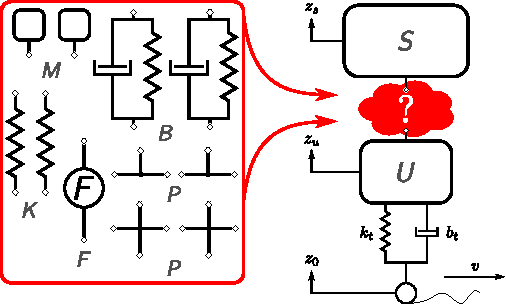
\includegraphics[width=0.6\columnwidth]{../ch2/figures/suspension1}
\caption{Suspension architecture enumeration case study.\label{fig:ch2:suspension1}}
\end{figure}

A graph representing a quarter-car suspension was introduced in Fig.~\ref{fig:ch2:initialexamples1}; now we will seek graphs that have different topologies between the sprung ($\xcolor{S}$) and unsprung ($\xcolor{U}$) masses represented in Fig.~\ref{fig:ch2:suspension1}. These graphs could then be used with design studies that evaluate the performance of a particular suspension architecture (see Ref.~\cite{Allison2014b} for a design study on a particular architecture).
The components considered will be additional masses, springs, dampers, a force actuator, and parallel connections (these are schematically shown in Fig.~\ref{fig:ch2:suspension1}). The specific selection of $(C,R,P)$ was chosen to be near the limits of what is currently possible with the proposed enumeration methods in this article.

Some additional assumptions are also made on the component definitions. First, $\xcolor{B}$ is a parallel damper and spring to ensure that there is a stable equilibrium point for the damper. Next, both 3- and 4-port parallel components are included to facilitate more efficient generation of the useful architectures. A 4-port parallel connection is equivalent to two 3-port parallel connections but the 4-port component provides structure that can be utilized with some specific NSCs. With the problem outlined, the base three-tuple is specified as:
\begin{gather*}
{C} = \{ \xcolor{S}, \xcolor{U}, \xcolor{M}, \xcolor{K}, \xcolor{B}, \xcolor{F}, \xcolor{P}, \xcolor{P} \}, \quad R =  [1,1,2,2,2,1,2,2] \\
{P} = [1,1,1,2,2,2,3,4], \quad N_P = 28, \quad N_C = 13 \\
1.01 \times 10^{7} \leq \abs*{\mathcal{G}_3} \leq 2.13 \times 10^{14}
\end{gather*}

The NSCs for this case study are now listed with expanded details on reduced potential adjacency matrix $A_R$. A few of the constraints utilize insights from the physical modeling of the suspension architectures.

\begin{enumerate}[label=$\bullet$, widest=$\bullet$, nosep]

\item \ref{ch2:s1}, \ref{ch2:s3} and \ref{ch2:s4} with $M = [1, 1, 0, 0, 0, 0, 0, 0]$ enforcing that both the sprung and unsprung masses must be connected and all components not connected to these two are removed.

\item \ref{ch2:s7} with $P$ as the number of unique edges.

\item $A_R(2,1) = 0$ for \ref{ch2:s5} to avoid a direct connection between the sprung and unsprung masses as it would defeat the purpose of a suspension to isolate the masses. If this constraint was not added, $1/27$ of graphs generated from a pure \mypm{} approach would contain this connection.

\item $A_R(3,1) = A_R(3,2) = 0$ for \ref{ch2:s5} since a feasible graph cannot have either $\xcolor{S}$ or $\xcolor{U}$ be connected to $\xcolor{M}$ as there would not be a path between between $\xcolor{S}$ and $\xcolor{U}$. Therefore, no unique graphs are lost with this constraint. Rather, a more efficient enumeration results.

\item $A_R(8,8) = A_R(7,7) = A_R(8,7) = 0$ for \ref{ch2:s5} so no parallel components can be connected to each other. This greatly reduces the number of graphs generated by providing some specific structure on the number and type of parallel connections in the architectures.

\item $A_R(4,4) = A_R(5,5) = 0$ for \ref{ch2:s5} so no two $\xcolor{K}$ or $\xcolor{B}$ components can be connected in series since there are straightforward relationships to combine these series elements into a single equivalent component. By eliminating this type of connection when generating graphs, we have a substantially smaller number of graphs to evaluate.

\item No parallel connection path can exist between a connected $\xcolor{S}$ or $\xcolor{U}$ as these masses would not be isolated. This is slightly different than the NSCs in Sec.~\ref{sec:ch2:NSC} and is checked after \ref{ch2:s5}.

\item Cycles appear with single parallel components where the components in the cycle would not appear in the dynamic model based on the properties of a parallel connection (e.g.,~with the cycle \resizebox{!}{0.03\columnwidth}{
\begin{tikzpicture}[
mynode/.style={draw, circle, very thick, inner sep=0.1pt, scale=1.3},
myline/.style={draw, very thick},
]
\node[mynode,draw=none] (1) at (0,0) {$\xcolor{P}$};
\node[mynode,draw=none] (2) at (0.8,0.3) {$\xcolor{K}$};
\node[mynode,draw=none] (3) at (1.6,0)  {$\xcolor{B}$};
\draw [myline] (1) -- (2);
\draw [myline] (1) -- (3);
\draw [myline] (2) -- (3);
\end{tikzpicture}}
, neither $\xcolor{K}$ nor $\xcolor{B}$ would appear in the dynamic model). Graphs with these cycles are declared unuseful since an isomorphic graph with the parallel cycle removed would already appear in the set of graphs generated by the tree algorithm.

\item Many series connections between the 2-port components are interchangeable (e.g.,~$\xcolor{F}-\xcolor{K}$ and $\xcolor{K}-\xcolor{F}$ in series are physically equivalent). Therefore, these interchangeable series components are combined into a single equivalent component type (modifying the graph) and checked for isomorphisms. For the previously mentioned example, the equivalent component type would be $\xcolor{FK}$ based on alphabetical ordering of the original component labels.

\end{enumerate}

The complete $A_R$ is shown in Fig.~\ref{fig:ch2:suspension2_1} and its expansion to the potential adjacency matrix in Fig.~\ref{fig:ch2:suspension2_2} noting that both of these matrices are symmetric. Figure~\ref{fig:ch2:suspension2_2} has $1$s on the diagonal since self-connections should be allowed so the desired graph structure space is covered. For example, we might want to consider graphs where all components are present except a single $\xcolor{K}$ component and this only can occur if the detached $\xcolor{K}$ is connected to itself (and later removed).

\begin{figure}
\centering
\begin{subfigure}[b]{\columnwidth}
\centering
\begin{align*}
% \scalemath{0.7}{
\scalemath{0.9}{
\begin{blockarray}{ccccccccc}
& \xcolor{S} & \xcolor{U} & \xcolor{M} & \xcolor{K} & \xcolor{B} & \xcolor{F} & \xcolor{P} & \xcolor{P} \\
\begin{block}{c[cccccccc]}
\xcolor{S} & 1 & \cdot & \cdot & \cdot & \cdot & \cdot & \cdot & \cdot \\
\xcolor{U} & \hlight{0}{20} & 1 & \cdot & \cdot & \cdot & \cdot & \cdot & \cdot \\
\xcolor{M} & \hlight{0}{55} & \hlight{0}{55} & 1 & \cdot & \cdot & \cdot & \cdot & \cdot  \\
\xcolor{K} & 1 & 1 & 1 & \hlight{0}{90} & \cdot & \cdot & \cdot & \cdot  \\
\xcolor{B} & 1 & 1 & 1 & 1 & \hlight{0}{90} & \cdot & \cdot & \cdot  \\
\xcolor{F} & 1 & 1 & 1 & 1 & 1 & 1 & \cdot & \cdot  \\
\xcolor{P} & 1 & 1 & 1 & 1 & 1 & 1 & \hlight{0}{37.5} & \cdot \\
\xcolor{P} & 1 & 1 & 1 & 1 & 1 & 1 & \hlight{0}{37.5} & \hlight{0}{37.5} \\
\end{block}
\end{blockarray}
}
\end{align*}
% \vspace{-0.35in}
\caption{Reduced potential adjacency matrix $A_R$.\label{fig:ch2:suspension2_1}}
% \vspace{0.1in}
\end{subfigure}
% 
\begin{subfigure}[b]{\columnwidth}
\vspace{0.3in}
\centering
\begin{align*}
% \scalemath{0.7}{
\scalemath{0.9}{
\begin{blockarray}{cccccccccccccc}
& \xcolor{S} & \xcolor{U} & \xcolor{M} & \xcolor{M} & \xcolor{K} & \xcolor{K} & \xcolor{B} & \xcolor{B} & \xcolor{F} & \xcolor{P} & \xcolor{P} & \xcolor{P} & \xcolor{P} \\
\begin{block}{c[ccccccccccccc]}
\xcolor{S} & \tikzmark{top}{1} & \cdot & \cdot & \cdot & \cdot & \cdot & \cdot & \cdot & \cdot & \cdot & \cdot & \cdot & \cdot \\
\xcolor{U} & \hlight{0}{20} & 1 & \cdot & \cdot & \cdot & \cdot & \cdot & \cdot & \cdot & \cdot & \cdot & \cdot & \cdot \\
\xcolor{M} &	\hlight{0}{55} & \hlight{0}{55} & 1 & \cdot & \cdot & \cdot & \cdot & \cdot & \cdot & \cdot & \cdot & \cdot & \cdot \\
\xcolor{M} &	\hlight{0}{55} & \hlight{0}{55} & 1 & 1 & \cdot & \cdot & \cdot & \cdot & \cdot & \cdot & \cdot & \cdot & \cdot \\
\xcolor{K} &	1 & 1 & 1 & 1 & 1 & \cdot & \cdot & \cdot & \cdot & \cdot & \cdot & \cdot & \cdot \\
\xcolor{K} &	1 & 1 & 1 & 1 & \hlight{0}{90} & 1 & \cdot & \cdot & \cdot & \cdot & \cdot & \cdot & \cdot \\
\xcolor{B} &	1 & 1 & 1 & 1 & 1 & 1 &	1 & \cdot & \cdot & \cdot & \cdot & \cdot & \cdot \\
\xcolor{B} &	1 & 1 & 1 & 1 & 1 & 1 &	\hlight{0}{90} & 1 & \cdot & \cdot & \cdot & \cdot & \cdot \\
\xcolor{F} &	1 & 1 & 1 & 1 & 1 & 1 &	1 & 1 & 1 & \cdot & \cdot & \cdot & \cdot \\
\xcolor{P} &	1 & 1 & 1 & 1 & 1 & 1 &	1 & 1 & 1 & 1 & \cdot & \cdot & \cdot \\
\xcolor{P} &	1 & 1 & 1 & 1 & 1 & 1 &	1 & 1 & 1 & \hlight{0}{37.5} & 1 & \cdot & \cdot \\
\xcolor{P} &	1 & 1 & 1 & 1 & 1 & 1 & 1 &	1 & 1 & \hlight{0}{37.5} & \hlight{0}{37.5} & 1 & \cdot \\
\xcolor{P} &	1 & 1 & 1 & 1 & 1 & 1 & 1 & 1 &	1 & \hlight{0}{37.5} & \hlight{0}{37.5} & \hlight{0}{37.5} & \tikzmark{bottom}{1}\ \\
\end{block}
\end{blockarray}
}
\end{align*}
\caption{Potential adjacency matrix.\label{fig:ch2:suspension2_2}}
\end{subfigure}
\caption{Suspension case study matrices for \ref{ch2:s5} and the tree search algorithm.\label{fig:ch2:suspension2}}
\end{figure}

The results are presented in similar manner to the previous case studies: $4.7\times 10^{21}$ adjacency matrices\footnote{This represents the fairest comparison as the proper permutations of the ports representation of the potential adjacency matrix in Fig.~\ref{fig:ch2:suspension2_2} without the parallel components. There are $5.4 \times 10^8$ adjacency matrices with a component representation but this suffers from the unknown parallel connection issue discussed in Sec.~\ref{sec:ch2:candidates}. There are $3.0 \times 10^{23}$ adjacency matrices directly using the matrix in Fig.~\ref{fig:ch2:suspension2}b.} ($\mathcal{G}_0$); $2.1 \times 10^{14}$ \mypm{}s ($\mathcal{G}_1$); $1.6 \times 10^8$ candidate graphs generated through the basic tree search algorithm; $3.2 \times 10^7$ remaining candidate graphs after initial port-type isomorphism filter; $1.9 \times 10^6$ feasible graphs ($\mathcal{G}_2$); and 13,727 unique graphs ($\mathcal{G}_3$). $2\times 10^{9}$ graph comparisons were needed and $3 \times 10^7$ required a full isomorphism check.
Two unique architectures are shown in Fig.~\ref{fig:ch2:suspension3} with Fig.~\ref{fig:ch2:suspension3_1} being a common architecture \cite{Allison2014b}.

\begin{figure}
\centering
\begin{subfigure}[b]{0.3\columnwidth}
\centering
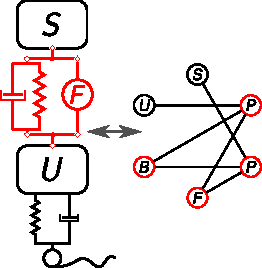
\includegraphics[width=\columnwidth]{../ch2/figures/suspension3_1}
\caption{\mypm{}~49073434464833.\label{fig:ch2:suspension3_1}}
\end{subfigure}
\begin{subfigure}[b]{0.35\columnwidth}
\centering
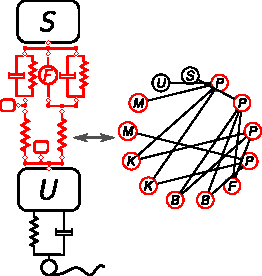
\includegraphics[width=\columnwidth]{../ch2/figures/suspension3_2}
\caption{\mypm{}~48728499790028.\label{fig:ch2:suspension3_2}}
\end{subfigure}
\caption{Two architectures for the suspension case study.\label{fig:ch2:suspension3}}
\end{figure}